%%%%%%%%%%%%%%%%%%%%%%%%%%%%%%%%%%%%
% スライドオプション
%%%%%%%%%%%%%%%%%%%%%%%%%%%%%%%%%%%%

% オプション1：解答あり（授業用）

\documentclass[t,compress,mathserif]{beamer}
\newcommand{\soln}[1]{\textit{#1}}
\newcommand{\solnGr}[1]{#1}

% オプション2：解答なし（配布用ハンドアウト）

%\documentclass[11pt,containsverbatim,handout]{beamer}
%\usepackage{pgfpages}
%\pgfpagesuselayout{4 on 1}[letterpaper,landscape,border shrink=5mm]
%\newcommand{\soln}[1]{ }
%\newcommand{\solnGr}{ }

%%%%%%%%%%%%%%%%%%%%%%%%%%%%%%%%%%%%
% 日本語サポート（LuaLaTeX使用）
% コンパイルコマンド: lualatex chp5.tex
%%%%%%%%%%%%%%%%%%%%%%%%%%%%%%%%%%%%

\usepackage{luatexja}
\usepackage{luatexja-fontspec}

%%%%%%%%%%%%%%%%%%%%%%%%%%%%%%%%%%%%
% スタイル
%%%%%%%%%%%%%%%%%%%%%%%%%%%%%%%%%%%%

\input{../lec_style_JP}

\setbeamertemplate{footline}{%
  \insertframenumber\,/\,\inserttotalframenumber}

%%%%%%%%%%%%%%%%%%%%%%%%%%%%%%%%%%%%
% プリアンブル
%%%%%%%%%%%%%%%%%%%%%%%%%%%%%%%%%%%%

\title[第5章：推測の基礎]{第5章：推測の基礎}
\author{OpenIntro Statistics 第4版（日本語版）}
\institute{$\:$ \\ {\footnotesize 原著スライド：Mine \c{C}etinkaya-Rundel（OpenIntro）\\
\webLink{http://creativecommons.org/licenses/by-sa/3.0/us/}{CC BY-SA ライセンス}のもと使用・翻訳。\\
一部の画像はフェアユース（教育目的）に基づき使用。}}
\date{}

%%%%%%%%%%%%%%%%%%%%%%%%%%%%%%%%%%%%
% ドキュメント開始
%%%%%%%%%%%%%%%%%%%%%%%%%%%%%%%%%%%%

\begin{document}


%%%%%%%%%%%%%%%%%%%%%%%%%%%%%%%%%%%%
% タイトルページ
%%%%%%%%%%%%%%%%%%%%%%%%%%%%%%%%%%%%

{
\addtocounter{framenumber}{-1}
{\removepagenumbers
\usebackgroundtemplate{
\includegraphics[width=\paperwidth]{../OpenIntro_Grid_4_3-01.jpg}}
\begin{frame}

\hfill 
\includegraphics[width=20mm]{../oiLogo_highres}

\titlepage

\end{frame}
}
}


%%%%%%%%%%%%%%%%%%%%%%%%%%%%%%%%%%%%
% 各節
%%%%%%%%%%%%%%%%%%%%%%%%%%%%%%%%%%%%

%%%%%%%%%%%%%%%%%%%%%%%%%%%%%%%%%%%%

\section{点推定値と標本変動性}

%%%%%%%%%%%%%%%%%%%%%%%%%%%%%%%%%%%%

\subsection{点推定値と誤差}

%%%%%%%%%%%%%%%%%%%%%%%%%%%%%%%%%%%%

\begin{frame}
\frametitle{点推定値と誤差}

\begin{itemize}

\item 私たちはしばしば\hl{母集団のパラメータ}（母数）に関心を持つ。

\item 母集団全体からデータを収集することは難しいため、未知の母集団パラメータの推定に\hl{標本統計量}を\hl{点推定値}として使用する。

\item 推定の\hl{誤差} ＝ 母集団パラメータと標本統計量の差

\item \hl{偏り（バイアス）}とは、真の母集団パラメータを系統的に過大または過小に推定する傾向のことである。

\item \hl{標本誤差}とは、ある標本から次の標本へと推定値がどれだけ変動しやすいかを表す。

\item 統計学の多くは標本誤差の理解と定量化に焦点を当てており、\hl{標本サイズ}はこの誤差を定量化するのに役立つ。

\end{itemize}

\end{frame}

%%%%%%%%%%%%%%%%%%%%%%%%%%%%%%%%%%%

\begin{frame}
\frametitle{}

\dq{アメリカの各州からそれぞれ1,000人の成人を無作為に抽出したとする。各州の身長の標本平均は同じになると思うか、やや異なると思うか、それとも大きく異なると思うか？}

\soln{同じではないが、それほど大きな差はなく、やや異なる程度だろう。}

\end{frame}

%%%%%%%%%%%%%%%%%%%%%%%%%%%%%%%%%%%%

\subsection{点推定値の変動性を理解する}

%%%%%%%%%%%%%%%%%%%%%%%%%%%%%%%%%%%%

\begin{frame}
\frametitle{}

\begin{center}

\includegraphics[width=0.95\textwidth]{5-1_point_est_sampling_var/figures/pew/pew1} \\
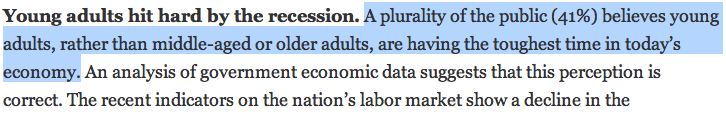
\includegraphics[width=0.95\textwidth]{5-1_point_est_sampling_var/figures/pew/pew2} \\
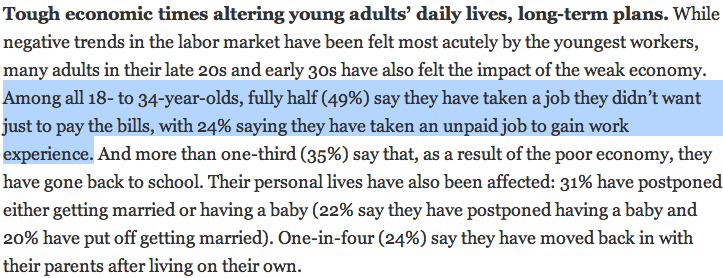
\includegraphics[width=0.95\textwidth]{5-1_point_est_sampling_var/figures/pew/pew3}
\end{center}

\ct{\webURL{http://pewresearch.org/pubs/2191/young-adults-workers-labor-market-pay-careers-advancement-recession}}

\end{frame}

%%%%%%%%%%%%%%%%%%%%%%%%%%%%%%%%%%%%

\begin{frame}
\frametitle{誤差の範囲（許容誤差）}

\begin{center}
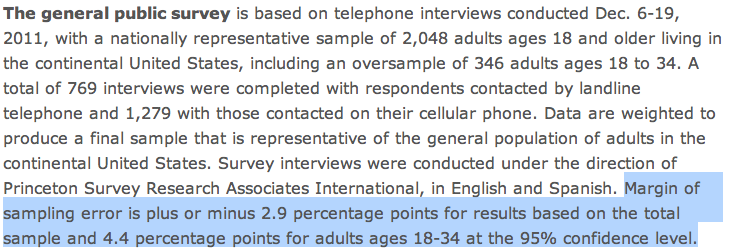
\includegraphics[width=0.95\textwidth]{5-1_point_est_sampling_var/figures/pew/pew4}
\end{center}

\begin{itemize}

\item 41\% $\pm$ 2.9\%：38.1\%から43.9\%の国民が、中年層や高齢者よりも若い成人が今日の経済で最も苦しんでいると考えていることを95\%の信頼度で確信している。

\item 49\% $\pm$ 4.4\%：18〜34歳の44.6\%から53.4\%が、請求書を支払うためだけに望まない仕事に就いたことがあると95\%の信頼度で確信している。

\end{itemize}

\end{frame}

%%%%%%%%%%%%%%%%%%%%%%%%%%%%%%%%%%%

\subsection{応用演習}

%%%%%%%%%%%%%%%%%%%%%%%%%%%%%%%%%%%

\begin{frame}
\frametitle{}

\dq{アメリカの成人で太陽光エネルギーの拡大を支持する割合が $p = 0.88$ であるとする（これが関心のあるパラメータである）。無作為に選ばれたアメリカの成人は、太陽光エネルギーの拡大を支持する可能性が高いか、低いか？}

\soln{より支持する可能性が高い。}

\end{frame}

%%%%%%%%%%%%%%%%%%%%%%%%%%%%%%%%

\begin{frame}
\frametitle{}

\dq{アメリカの成人全体の母集団にアクセスできない場合（これはよくある状況である）、太陽光エネルギーの拡大を支持するアメリカの成人の割合を推定するために、母集団から標本を抽出し、その標本割合を未知の母集団割合の最良の推定値として使用することが考えられる。}

\begin{itemize}

\item 母集団からアメリカの成人1,000人を復元抽出し、太陽光エネルギーの拡大を支持するかどうかを記録する。

\item 標本割合を求める。

\item クラスの各メンバーが得た標本割合の分布をプロットする。

\end{itemize}

\end{frame}

%%%%%%%%%%%%%%%%%%%%%%%%%%%%%%%%%%%

\begin{frame}[fragile]
\frametitle{}

\begin{beamerboxesrounded}[shadow = true, lower = code body]{}
{
\small
\begin{verbatim}

# 1. Create a set of 250 million entries, where 88% of
# them are "support" and 12% are "not".

pop_size <- 250000000
possible_entries <- c(rep("support", 0.88 * pop_size),
                      rep("not", 0.12 * pop_size))


# 2. Sample 1000 entries without replacement.

sampled_entries <- sample(possible_entries, size = 1000)

# 3. Compute p-hat: count the number that are "support",
# then divide by # the sample size.

sum(sampled sampled_entries == "support") / 1000

\end{verbatim}
}
\end{beamerboxesrounded}

\end{frame}

%%%%%%%%%%%%%%%%%%%%%%%%%%%%%%%%%%%

\begin{frame}
\frametitle{標本分布}

このプロセスを何度も繰り返して多くの $\hat{p}$ を得たとする。この分布を\hl{標本分布}と呼ぶ。

\begin{center}
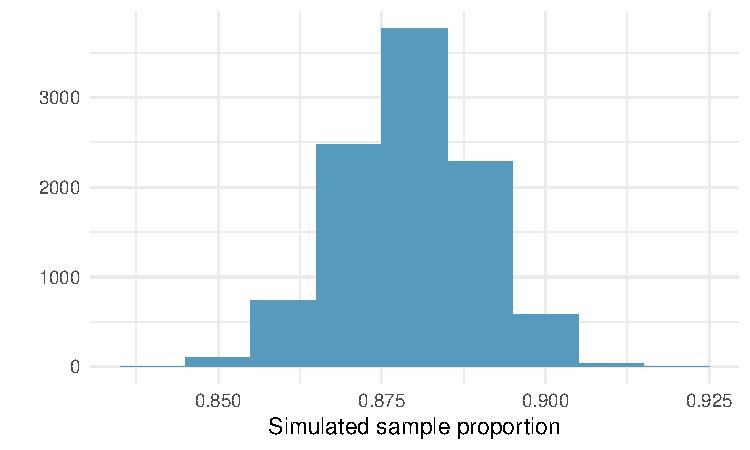
\includegraphics[width=0.6\textwidth]{5-1_point_est_sampling_var/figures/solar-power/solar-power-sampling.pdf}
\end{center}

\end{frame}

%%%%%%%%%%%%%%%%%%%%%%%%%%%%%%%%%%%

\begin{frame}
\frametitle{}

\dq{この分布の形と中心はどのようなものか？この分布に基づいて、真の母集団割合はどれくらいだと思うか？}

\begin{center}
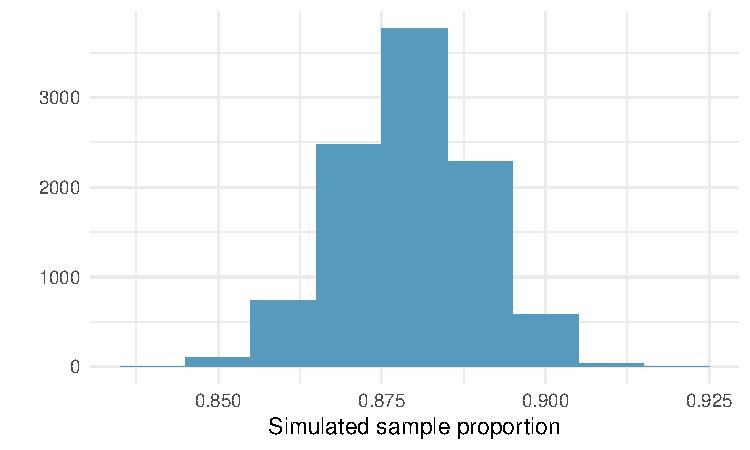
\includegraphics[width=0.6\textwidth]{5-1_point_est_sampling_var/figures/solar-power/solar-power-sampling.pdf}
\end{center}

$\:$ \\
\soln{この分布は単峰性でほぼ対称である。真の母集団割合の合理的な推測は、この分布の中心で、約0.88である。}

\end{frame}

%%%%%%%%%%%%%%%%%%%%%%%%%%%%%%%%

\begin{frame}
\frametitle{標本分布は実際には観察されない}

\begin{itemize}

\item 実際の応用では、標本分布を直接観察することは決してないが、点推定値はそのような仮想的な分布から得られるものとして常に考えることが有用である。

\item 標本分布を理解することで、実際に観察する点推定値の特性を明らかにし、理解することができる。

\end{itemize}

\end{frame}

%%%%%%%%%%%%%%%%%%%%%%%%%%%%%%%%

\subsection{中心極限定理}

%%%%%%%%%%%%%%%%%%%%%%%%%%%%%%%%%%

\begin{frame}
\frametitle{中心極限定理}

\formula{中心極限定理}
{標本割合は、母集団の割合 $p$ を平均とし、標準誤差を $\sqrt{\frac{p~(1-p)}{n}}$ とする正規分布にほぼ従う。
\[ \hat{p} \sim N \pr{ \text{平均} = p, SE = \sqrt{\frac{p~(1-p)}{n}} } \]
}

\begin{itemize}

\item 先ほど見た標本分布が対称で真の母集団割合を中心としていたことは偶然ではなかった。

\item $SE = \sqrt{\frac{p~(1-p)}{n}}$ の詳細な証明は省くが、$n$ が増加すると $SE$ が減少することに注目されたい。
\begin{itemize}
\item $n$ が増えるにつれて、標本はより一貫した $\hat{p}$ をもたらし、すなわち $\hat{p}$ 間の変動性が低くなる。
\end{itemize}

\end{itemize}

\end{frame}

%%%%%%%%%%%%%%%%%%%%%%%%%%%%%%%%%%%%

\begin{frame}
\frametitle{中心極限定理の適用条件}

中心極限定理を適用するためには、一定の条件が満たされなければならない：

\begin{enumerate}

\item \hlGr{独立性：}抽出された観測値は互いに独立でなければならない。\\

これを確認することは難しいが、以下の場合により可能性が高い：
\begin{itemize}
\item 無作為抽出・割り当てが行われている場合、および
\item 非復元抽出の場合、$n$ が母集団の10\%未満である場合。
\end{itemize}

\item \hlGr{標本サイズ：}観察された標本において、期待される成功数と失敗数がそれぞれ少なくとも10以上あること。

母集団割合が不明な場合（または仮定できない場合）、この条件を確認することは難しい。そのような場合は、観察された成功数と失敗数がそれぞれ少なくとも10以上あることを確認する。

\end{enumerate}

\end{frame}
%%%%%%%%%%%%%%%%%%%%%%%%%%%%%%%%%%

\subsection{中心極限定理の実際への応用}

%%%%%%%%%%%%%%%%%%%%%%%%%%%%%%%%%%

\begin{frame}
\frametitle{$p$ が未知の場合}

\begin{itemize}

\item 中心極限定理では $SE = \sqrt{\frac{p~(1-p)}{n}}$ とされており、$np$ と $n(1-p)$ がそれぞれ少なくとも10であることが条件だが、母集団割合 $p$ の値が不明なことが多い。

\item そのような場合は $p$ の代わりに $\hat{p}$ を代入する。

\end{itemize}

\end{frame}

%%%%%%%%%%%%%%%%%%%%%%%%%%%%%%%%%%%

\subsection{中心極限定理に関するさらなる詳細}

%%%%%%%%%%%%%%%%%%%%%%%%%%%%%%%%%%%%

\begin{frame}
\frametitle{$p$ が小さい場合}

\dq{真の母集団割合が $p = 0.05$ である母集団があり、この母集団からサイズ $n = 50$ の無作為標本を抽出するとする。各標本の標本割合を計算してこれらの割合をプロットした場合、この分布はほぼ正規分布になると予想されるか？なぜそうなるか、あるいはならないか？}

\soln{いいえ、成功・失敗条件が満たされていないため（$50 \times 0.05 = 2.5$）、標本分布がほぼ正規分布になるとは期待できない。
\begin{center}
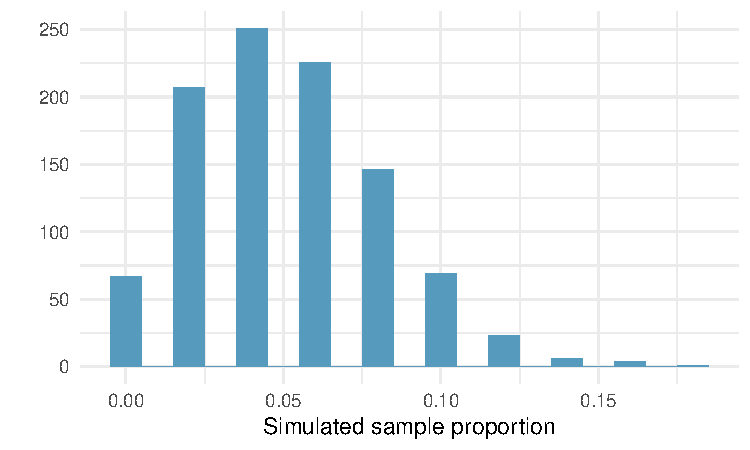
\includegraphics[width=0.55\textwidth]{5-1_point_est_sampling_var/figures/sf/low-p.pdf}
\end{center}
}

\end{frame}

%%%%%%%%%%%%%%%%%%%%%%%%%%%%%%%%%%%

\begin{frame}

\dq{$np$ および/または $n(1-p)$ が10未満の場合はどうなるか？}

\begin{center}
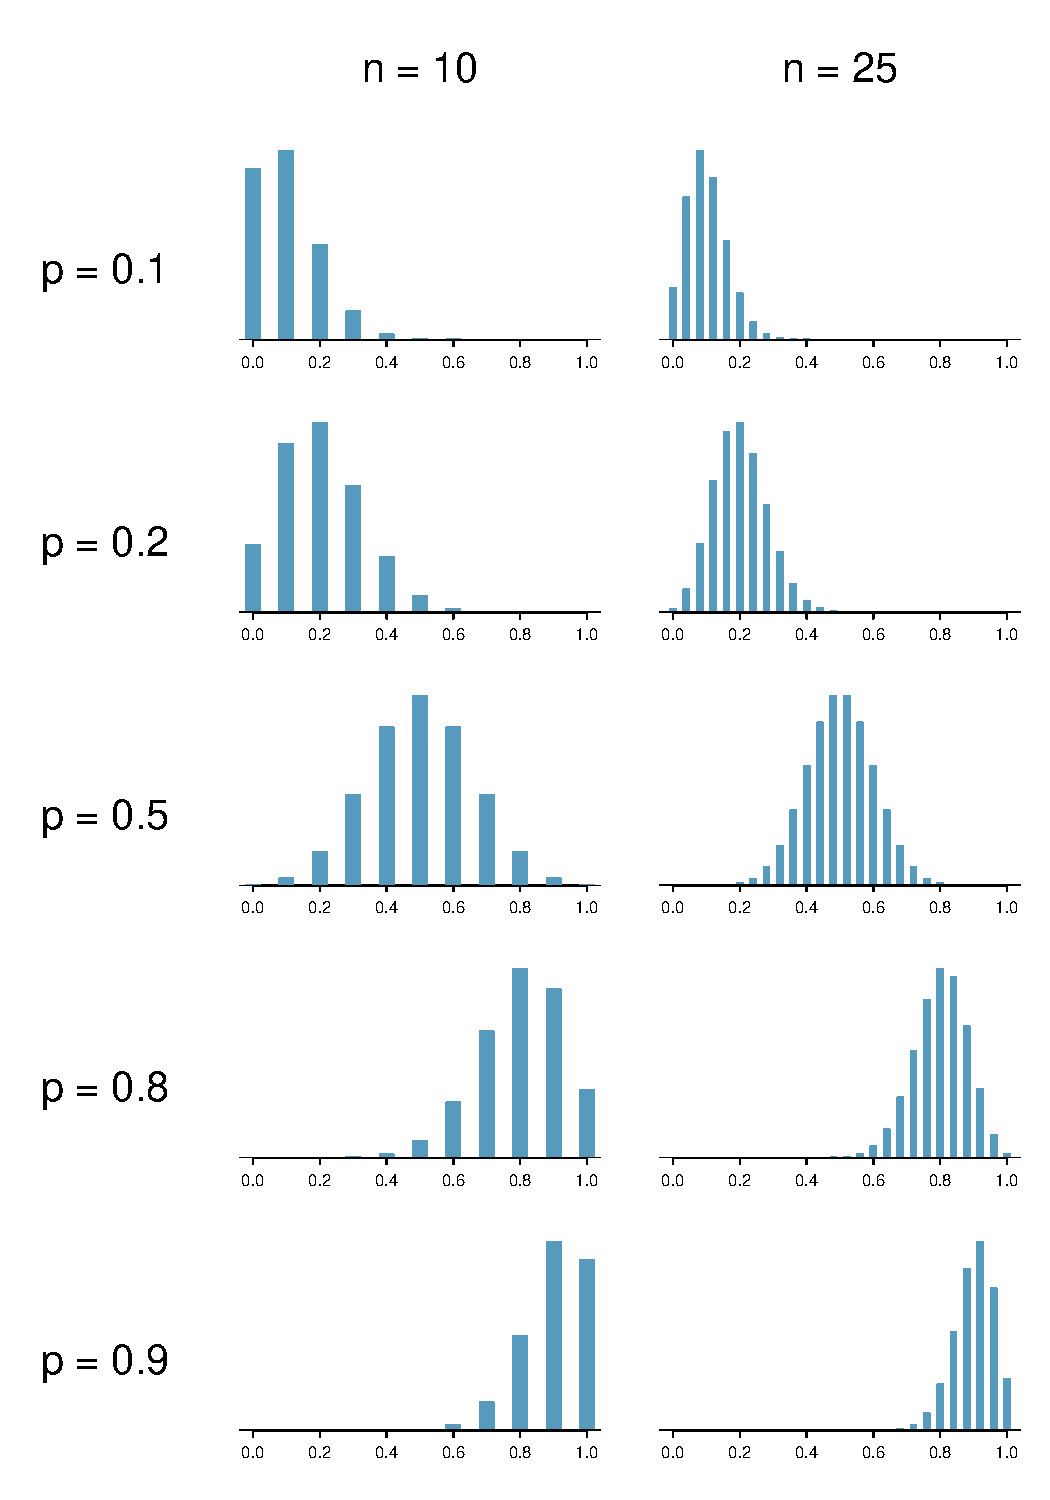
\includegraphics[width=0.45\textwidth]{5-1_point_est_sampling_var/figures/clt_prop_grid/clt_prop_grid_1.pdf}
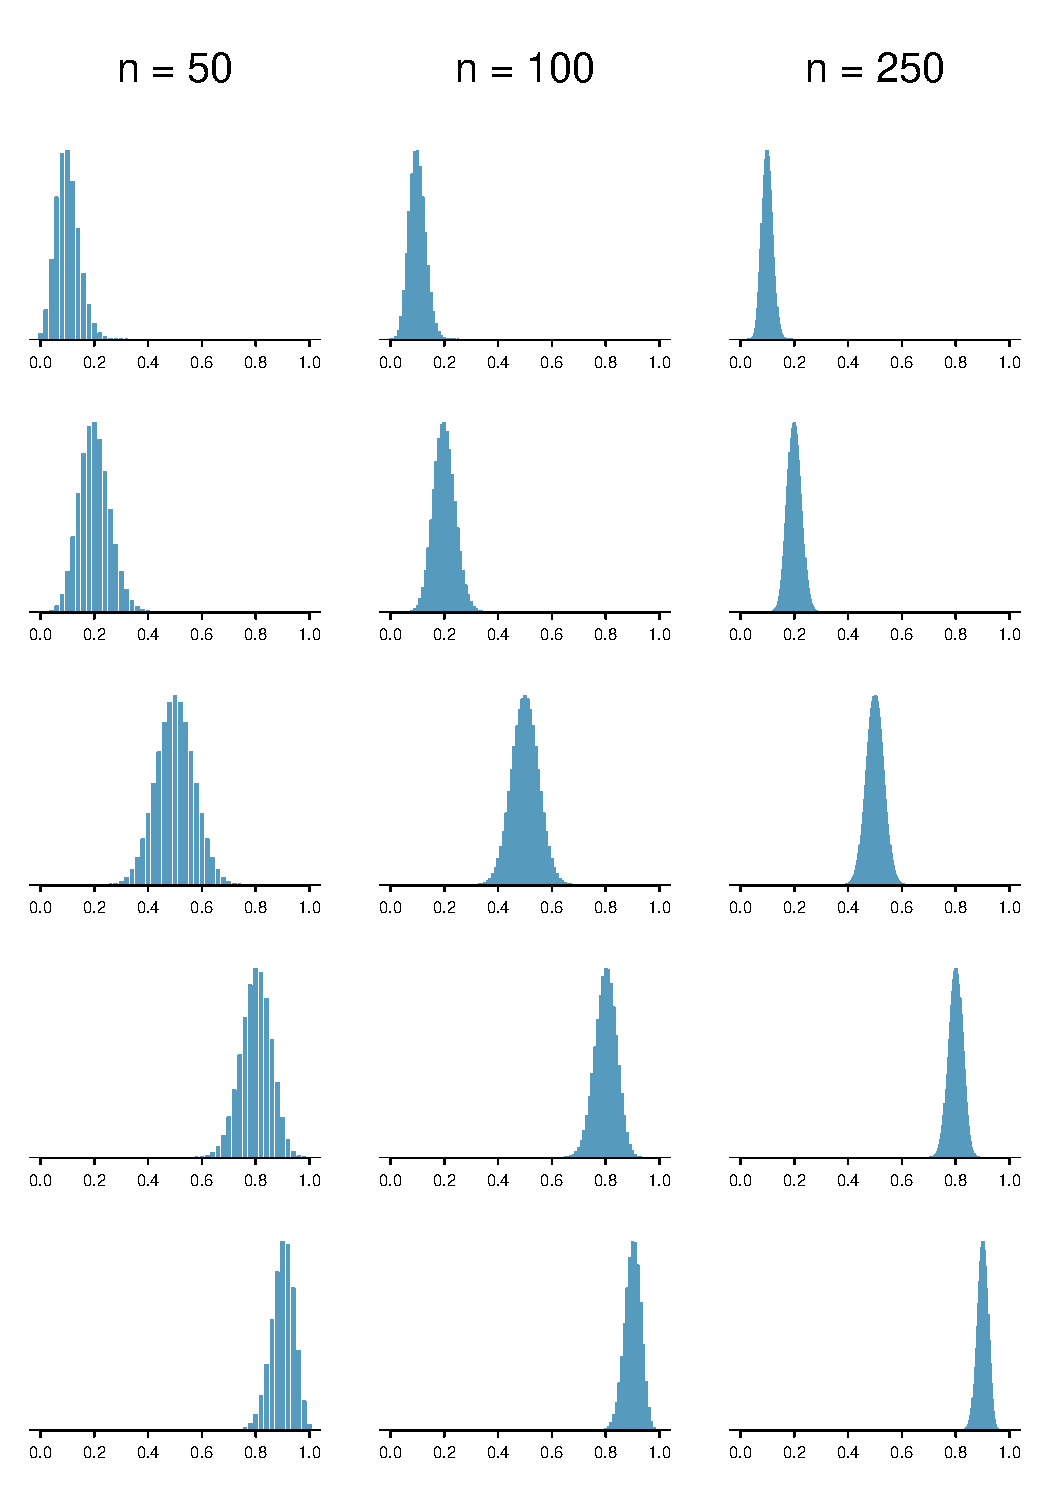
\includegraphics[width=0.45\textwidth]{5-1_point_est_sampling_var/figures/clt_prop_grid/clt_prop_grid_2.pdf}
\end{center}

\end{frame}

%%%%%%%%%%%%%%%%%%%%%%%%%%%%%%%%%%%

\begin{frame}
\frametitle{条件が満たされない場合…}

\begin{itemize}

\item $np$ または $n(1-p)$ のいずれかが小さい場合、分布はより離散的になる。
\item $np$ または $n(1-p)$ が10未満の場合、分布はよりゆがんだ形になる。
\item $np$ と $n(1-p)$ の両方が大きくなるほど、分布はより正規分布に近くなる。
\item $np$ と $n(1-p)$ の両方が非常に大きい場合、分布の離散性はほとんど見られなくなり、分布は正規分布にかなり近い形になる。

\end{itemize}

\end{frame}

%%%%%%%%%%%%%%%%%%%%%%%%%%%%%%%%%%%%

\subsection{他の統計量への枠組みの拡張}

%%%%%%%%%%%%%%%%%%%%%%%%%%%%%%%%%%%%

\begin{frame}
\frametitle{他の統計量への枠組みの拡張}

\begin{itemize}

\item 標本統計量を使ってパラメータを推定するという戦略は非常に一般的であり、割合以外の統計量にも適用できる戦略である。

\begin{itemize}
\item 大学の学生の無作為標本を抽出し、課外活動にいくつ参加しているかを聞いて、その大学の全学生が参加している課外活動の平均数を推定する。
\end{itemize}

\item この章の原則と一般的な考え方は、詳細が若干変わるとしても、他のパラメータにも適用される。

\end{itemize}

\end{frame}

%%%%%%%%%%%%%%%%%%%%%%%%%%%%%%%%%%%%

\section{割合の信頼区間}

%%%%%%%%%%%%%%%%%%%%%%%%%%%%%%%%%%%%

\subsection{母集団パラメータの捕捉}

%%%%%%%%%%%%%%%%%%%%%%%%%%%%%%%%%%%%

\begin{frame}[shrink]
\frametitle{信頼区間}

\begin{itemize}

\item 母集団パラメータの妥当な値の範囲を\hl{信頼区間}と呼ぶ。

\item 標本統計量だけを使ってパラメータを推定することは、濁った湖で銛を使って魚を突こうとするようなものであり、信頼区間を使うことは網を使って魚を捕まえようとするようなものである。
$\:$ \\
$\:$ \\
\begin{columns}[c]
\column{0.25\textwidth}
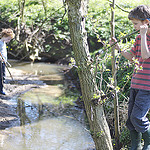
\includegraphics[width=\textwidth]{5-2_ci_prop/figures/spear}
\column{0.5\textwidth}
{\small
魚を見た場所に銛を投げても、たいていは外れてしまう。その辺りに網を投げれば、魚を捕まえる可能性が高い。
}
\column{0.25\textwidth}
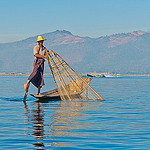
\includegraphics[width=\textwidth]{5-2_ci_prop/figures/net}
\end{columns}
$\:$ \\
\item 点推定値を報告しても、正確な母集団パラメータには当たらないかもしれない。妥当な値の範囲を報告すれば、パラメータを捉える可能性が高くなる。

\end{itemize}

{\tiny 写真提供：Mark Fischer (http://www.flickr.com/photos/fischerfotos/7439791462) および Chris Penny (http://www.flickr.com/photos/clearlydived/7029109617) on Flickr.}

\end{frame}

%%%%%%%%%%%%%%%%%%%%%%%%%%%%%%%%%%%%

\subsection{95\%信頼区間の構築}

%%%%%%%%%%%%%%%%%%%%%%%%%%%%%%%%%%%%

\begin{frame}
\frametitle{Facebookによるユーザー興味分類}

\dq{多くの商業ウェブサイト（ソーシャルメディアプラットフォーム、ニュースサイト、オンライン小売業者など）はユーザーの行動データを収集し、ターゲットを絞ったコンテンツ、おすすめ、広告の配信に活用している。アルゴリズムによる分類システムがアメリカ人の実際の生活をどの程度反映しているかを理解するため、ピュー・リサーチはアメリカのFacebookユーザー850人の代表的な標本に対し、Facebookの「興味のあるもの」ページに表示されたカテゴリーが自分や自分の興味を正確に表しているかどうかを尋ねた。回答者の67\%が、表示されたカテゴリーは正確だと答えた。Facebookが自分の興味を正確に分類していると思うアメリカのFacebookユーザーの真の割合を推定せよ。}

\ct{\webURL{https://www.pewinternet.org/2019/01/16/facebook-algorithms-and-personal-data/}}

\end{frame}

%%%%%%%%%%%%%%%%%%%%%%%%%%%%%%%%%%%%

\begin{frame}
\frametitle{Facebookによるユーザー興味分類}

\[ \hat{p} = 0.67 \qquad n = 850 \]

おおよその95\%信頼区間は次のように定義される：
\[ \text{点推定値} \pm 1.96 \times SE \]

\vspace{-0.25cm}
\[ SE = \sqrt{\frac{p(1-p)}{n}} = \sqrt{\frac{0.67 \times 0.33}{850}} \approx 0.016 \]

\vspace{-0.25cm}
\begin{eqnarray*}
\hat{p} \pm 1.96 \times SE &=& 0.67 \pm 1.96 \times 0.016 \\
&=& (0.67 - 0.03, 0.67 + 0.03) \\
&=& (0.64, 0.70)
\end{eqnarray*}


\end{frame}

%%%%%%%%%%%%%%%%%%%%%%%%%%%%%%%%%%%

\begin{frame}
\frametitle{}

\pq{この信頼区間の正しい解釈はどれか？}

95\%の確信を持って言えることは：
\begin{enumerate}[(a)]
\item この標本のアメリカのFacebookユーザーの64\%から70\%が、Facebookは自分の興味を正確に分類していると思っている。
\solnMult{アメリカのFacebookユーザー全体の64\%から70\%が、Facebookは自分の興味を正確に分類していると思っている}
\item 無作為に選ばれたアメリカのFacebookユーザーの興味が正確に分類されている確率が64\%から70\%である。
\item アメリカのFacebookユーザーの95\%の興味が正確に分類されている確率が64\%から70\%である。
\end{enumerate}

\end{frame}

%%%%%%%%%%%%%%%%%%%%%%%%%%%%%%%%%%%

\begin{frame}
\frametitle{「95\%の確信」とはどういう意味か？}

\begin{itemize}

\item 多くの標本を抽出し、$\text{点推定値} \pm 1.96 \times SE$ という式を使って各標本から信頼区間を構築したとする。

\item すると、その区間の約95\%が真の母集団割合（$p$）を含むことになる。

\end{itemize}

\end{frame}

%%%%%%%%%%%%%%%%%%%%%%%%%%%%%%%%%%%

\begin{frame}
\frametitle{区間の幅}

\dq{母集団パラメータをより確実に捉えたい場合、すなわち信頼水準を高めたい場合、より広い区間を使うべきか、それとも狭い区間を使うべきか？}

\soln{より広い区間。}

$\:$ \\

\dq{より広い区間を使うことの欠点はあるか？}
\begin{center}

\includegraphics[width=0.9\textwidth]{5-2_ci_prop/figures/garfield}
\end{center}

\soln{区間が広すぎると、あまり有用な情報が得られないかもしれない。}

{\scriptsize 画像出典：http://web.as.uky.edu/statistics/users/earo227/misc/garfield\_weather.gif}

\end{frame}

%%%%%%%%%%%%%%%%%%%%%%%%%%%%%%%%%%%

\subsection{信頼水準の変更}

%%%%%%%%%%%%%%%%%%%%%%%%%%%%%%%%%%%

\begin{frame}
\frametitle{信頼水準の変更}

\[ \text{点推定値} \pm z^\star \times SE \]

\begin{itemize}

\item 信頼区間において、$z^\star \times SE$ を\hl{誤差の範囲（許容誤差）}と呼び、ある標本に対して、信頼水準が変わると許容誤差も変わる。

\item 信頼水準を変えるには、上の式の $z^\star$ を調整する必要がある。

\item 実際によく使われる信頼水準は90\%、95\%、98\%、99\%である。

\item 95\%信頼区間では、$z^\star = 1.96$ である。

\item ただし、標準正規（$z$）分布を使えば、任意の信頼水準に対応する適切な $z^\star$ を求めることができる。

\end{itemize}

\end{frame}

%%%%%%%%%%%%%%%%%%%%%%%%%%%%%%%%%%%%

\begin{frame}

\pq{98\%信頼区間を計算する際の適切な $z^\star$ はどのZ値か？}

\begin{multicols}{2}
\begin{enumerate}[(a)]
\item $Z = 2.05$
\item $Z = 1.96$
\solnMult{$Z = 2.33$}
\item $Z = -2.33$
\item $Z = -1.65$
\item[]
\end{enumerate}
\end{multicols}

\soln{
\begin{center}
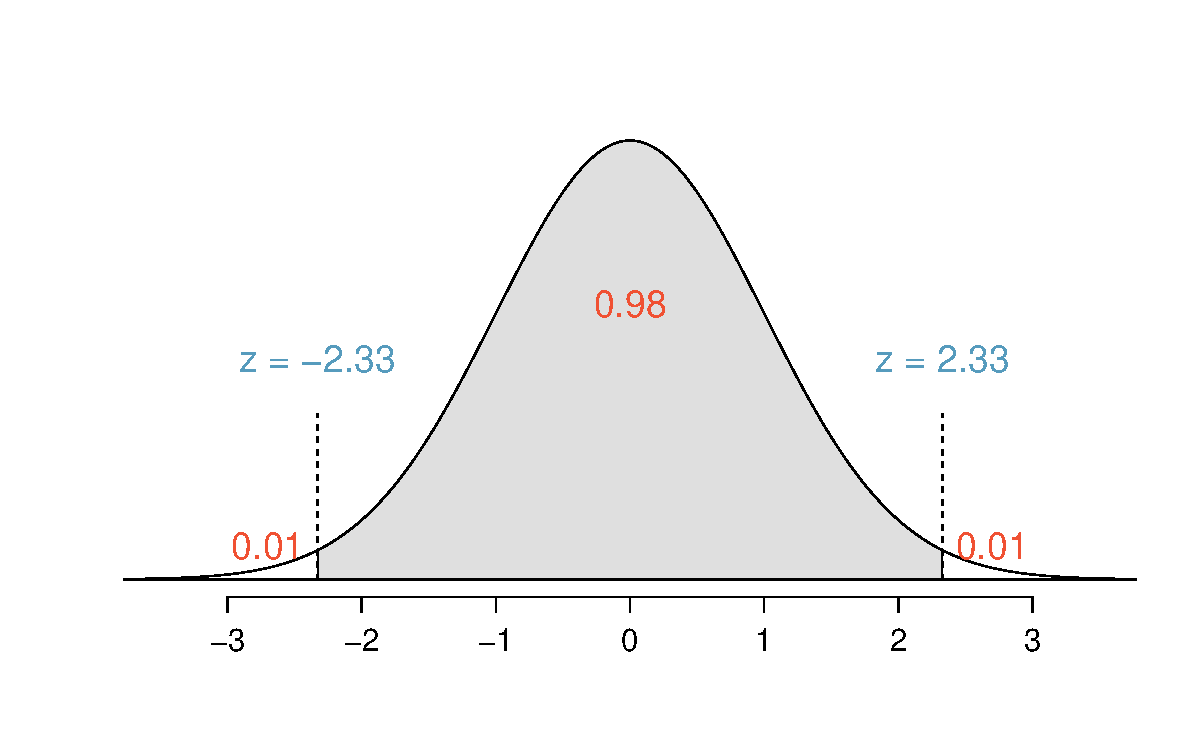
\includegraphics[width=0.7\textwidth]{5-2_ci_prop/figures/middle98/middle98}
\end{center}
}

\end{frame}

%%%%%%%%%%%%%%%%%%%%%%%%%%%%%%%%%%%

\subsection{信頼区間の解釈}

%%%%%%%%%%%%%%%%%%%%%%%%%%%%%%%%%%%

\begin{frame}
\frametitle{信頼区間の解釈}

信頼区間は…

\begin{itemize}

\item 常に母集団についてのものである

\item 確率の陳述ではない

\item 個々の観測値ではなく、母集団パラメータのみについてのものである

\item 基となる標本統計量が母集団パラメータの不偏推定量である場合にのみ信頼できる

\end{itemize}

\end{frame}

%%%%%%%%%%%%%%%%%%%%%%%%%%%%%%%%%%%

%%%%%%%%%%%%%%%%%%%%%%%%%%%%%%%%%%%%

\section{割合の仮説検定}

%%%%%%%%%%%%%%%%%%%%%%%%%%%%%%%%%%%%

\subsection{仮説検定の枠組み}

%%%%%%%%%%%%%%%%%%%%%%%%%%%%%%%%%%%%

\begin{frame}
\frametitle{思い出してみよう…}

性差別実験：

{\footnotesize
\begin{tabular}{ll  cc c}
  		&				& \multicolumn{2}{c}{\textit{昇進}} \\
\cline{3-4}
							&			& 昇進あり	& 昇進なし	& 合計	\\
\cline{2-5}
\multirow{2}{*}{\textit{性別}}	&男性		& 21	 	& 3		& 24 	\\
							&女性		& 14	 	& 10 	 	& 24 \\
\cline{2-5}
							&合計		& 35		& 13		& 48 \\
\end{tabular}
}

\[ \hat{p}_{\text{男性}} = 21 / 24 \approx 0.88 ~ \text{ および } ~ \hat{p}_{\text{女性}} = 14 / 24 \approx 0.58 \]

考えられる説明：
\begin{itemize}
\item 昇進と性別は\hl{独立}であり、性差別はなく、割合の差は単なる偶然による。$\rightarrow$ \orange{帰無仮説} - {\small （何も起きていない）}
\item 昇進と性別は\hl{従属}であり、性差別があり、割合の差は偶然ではない。$\rightarrow$ \orange{対立仮説} - {\small （何かが起きている）}

\end{itemize}

\end{frame}

%%%%%%%%%%%%%%%%%%%%%%%%%%%%%%%%%%%%

\begin{frame}
\frametitle{結果}

\begin{center}
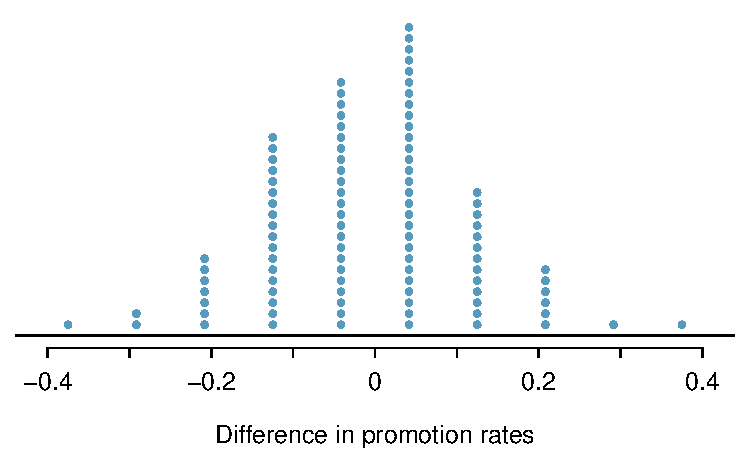
\includegraphics[width=0.75\textwidth]{5-3_ht_prop/figures/discRandDotPlot/discRandDotPlot}
\end{center}

シミュレーションにおいて実際のデータと同等またはそれ以上の極端な結果（男性の昇進率が女性より30\%以上高い）が得られる可能性は非常に低かったため、帰無仮説を棄却して対立仮説を採択することにした。

\end{frame}

%%%%%%%%%%%%%%%%%%%%%%%%%%%%%%%%%%%%

\begin{frame}
\frametitle{まとめ：仮説検定の枠組み}

\begin{itemize}
\item 現状を表す\hl{帰無仮説（$H_0$）}から始める。
\item また、研究上の問い（検定したいこと）を表す\hl{対立仮説（$H_A$）}も設定する。
\item 帰無仮説が真であるという前提のもとで、シミュレーションまたは中心極限定理に基づく伝統的な手法によって仮説検定を行う（次に説明する）。
\item 検定結果が、対立仮説を支持する説得力のある証拠がデータに含まれないことを示す場合は、帰無仮説を維持する。そうでない場合は、帰無仮説を棄却して対立仮説を採択する。
\end{itemize}
割合に関する主張を検定する例を使って、仮説検定の枠組みを正式に紹介する。

\end{frame}

%%%%%%%%%%%%%%%%%%%%%%%%%%%%%%%%%%%

\subsection{信頼区間を用いた仮説検定}

%%%%%%%%%%%%%%%%%%%%%%%%%%%%%%%%%%%%

\begin{frame}
\frametitle{信頼区間を用いた仮説検定}

{\small \dq{先ほど、Facebookが自分の興味を正確に分類していると思うアメリカのFacebookユーザーの割合に対する95\%信頼区間を64\%から67\%と計算した。この信頼区間に基づいて、アメリカのFacebookユーザーの過半数がFacebookによる興味の分類は正確だと思っているという仮説をデータは支持するか？}}

\begin{itemize}

\item 対応する仮説は次の通りである：
\begin{itemize}
\item[$H_0$:] $p = 0.50$：アメリカのFacebookユーザーの50\%がFacebookによる興味の分類は正確だと思っている
\item[$H_A$:] $p > 0.50$：アメリカのFacebookユーザーの50\%以上がFacebookによる興味の分類は正確だと思っている
\end{itemize}

\item 帰無値が区間に含まれていない $\rightarrow$ 帰無仮説を棄却する。

\item これは仮説検定の簡便な方法だが、帰無仮説のもとでの特定の結果の可能性（p値）は示さない。

\end{itemize}

\end{frame}

%%%%%%%%%%%%%%%%%%%%%%%%%%%%%%%%%%%%

\subsection{決定誤差}

%%%%%%%%%%%%%%%%%%%%%%%%%%%%%%%%%%%%

\begin{frame}
\frametitle{決定誤差}

\begin{itemize}

\item 仮説検定は完璧ではない。

\item 司法制度では、無実の人が誤って有罪判決を受けたり、有罪の人が無罪放免になったりすることがある。

\item 同様に、統計的仮説検定でも誤った決定をすることがある。

\item 違いは、統計学では誤りを犯す頻度を定量化するための道具があることである。

\end{itemize}

\end{frame}

%%%%%%%%%%%%%%%%%%%%%%%%%%%%%%%%%%%%

\begin{frame}
\frametitle{決定誤差（続き）}

帰無仮説と対立仮説という2つの競合する仮説がある。仮説検定では、どちらが真である可能性が高いかを決定するが、その選択が誤っている場合がある。\\

\begin{center}
\begin{tabular}{l l | c c}
\multicolumn{2}{c}{} & \multicolumn{2}{c}{\textbf{決定}} \\
& & $H_0$ を棄却しない &  $H_0$ を棄却する \\
  \cline{2-4}
& $H_0$ が真 & \green{$\checkmark$} &  \orange{第一種の過誤} \\
\raisebox{1.5ex}{\textbf{真実}} & $H_A$ が真 & \orange{第二種の過誤} & \green{$\checkmark$} \\
  \cline{2-4}
\end{tabular}
\end{center}

\begin{itemize}
\item \hl{第一種の過誤}とは、$H_0$ が真であるときに帰無仮説を棄却することである。

\item \hl{第二種の過誤}とは、$H_A$ が真であるときに帰無仮説を棄却しないことである。

\item $H_0$ または $H_A$ のどちらが真であるかは（ほぼ）わからないが、すべての可能性を考慮する必要がある。

\end{itemize}

\end{frame}

%%%%%%%%%%%%%%%%%%%%%%%%%%%%%%%%%%%%

\begin{frame}[shrink]
\frametitle{仮説検定を裁判として考える}

仮説検定を刑事裁判として考えると、帰無仮説と対立仮説の観点から評決を組み立てることが理にかなっている：
\begin{align*}
H_0&：\text{被告は無実である} \\
H_A&：\text{被告は有罪である}
\end{align*}

次の状況ではどの種類の誤りが犯されているか？

\begin{itemize}
\item 実際には有罪の被告を無実と宣告する
\soln{\begin{center}\hl{第二種の過誤}\end{center}}
\item 実際には無実の被告を有罪と宣告する
\soln{\begin{center}\hl{第一種の過誤}\end{center}}
\end{itemize}

どちらの誤りがより深刻だと思うか？
\begin{center}{\footnotesize 「10人の有罪者を逃がすことは、1人の無実の人を苦しめることより好ましい」\\ ——ウィリアム・ブラックストーン}\end{center}
\end{frame}

%%%%%%%%%%%%%%%%%%%%%%%%%%%%%%%%%%%%

\begin{frame}
\frametitle{第一種の過誤の確率}

\begin{itemize}

\item 一般的なルールとして、p値が0.05未満のとき $H_0$ を棄却する。すなわち、\hl{有意水準} 0.05、\mathhl{\alpha = 0.05} を使用する。

\item これは、$H_0$ が実際に真である場合に、5\%を超えて誤って棄却したくないということを意味する。

\item 言い換えると、5\%の有意水準を使用する場合、帰無仮説が真であれば第一種の過誤を犯す確率は約5\%である。
\[ \mathhl{ P(\text{第一種の過誤} \: | \: \text{$H_0$ が真}) = \alpha } \]

\item これが $\alpha$ の小さい値を好む理由である。$\alpha$ を大きくすると第一種の過誤の確率が高まる。

\end{itemize}

\end{frame}

%%%%%%%%%%%%%%%%%%%%%%%%%%%%%%%%%%%%

\subsection{p値を用いた正式な検定}

%%%%%%%%%%%%%%%%%%%%%%%%%%%%%%%%%%%%

\begin{frame}
\frametitle{Facebookの興味カテゴリー}

\dq{同じ調査で850人の回答者に対し、Facebookが自分のカテゴリーリストを作成することにどの程度快適に感じるかを尋ねた。回答者の41\%が快適だと答えた。Facebookが自分の興味カテゴリーリストを作成することに快適に感じるアメリカのFacebookユーザーの割合が50\%と異なるという説得力のある証拠をこのデータは提供しているか？}

\vfill

\ct{\webURL{https://www.pewinternet.org/2019/01/16/facebook-algorithms-and-personal-data/}}

\end{frame}

%%%%%%%%%%%%%%%%%%%%%%%%%%%%%%%%%%

\begin{frame}
\frametitle{仮説の設定}

\begin{itemize}

\item \hl{関心のあるパラメータ}は、Facebookが自分の興味カテゴリーを作成することに快適に感じる\underline{すべての}アメリカのFacebookユーザーの割合である。

\item 標本割合が0.50（少数派）より低い理由として、2つの説明が考えられる：
\begin{itemize}
\item 真の母集団割合が0.50と異なる。
\item 真の母集団割合は0.50であり、真の母集団割合と標本割合の差は単なる自然な標本変動性によるものである。
\end{itemize}

\end{itemize}

\end{frame}

%%%%%%%%%%%%%%%%%%%%%%%%%%%%%%%%%%

\begin{frame}
\frametitle{仮説の設定}

\begin{itemize}

\item アメリカのFacebookユーザーの50\%がFacebookによる興味カテゴリーの作成に快適に感じているという仮定から始める：
\[ \mathhl{H_0:}~p = 0.50 \]

\item Facebookによる興味カテゴリーの作成に快適に感じるアメリカのFacebookユーザーの割合が50\%と異なるという主張を検定する：
\[ \mathhl{H_A:}~p \ne 0.50 \]

\end{itemize}

\end{frame}

%%%%%%%%%%%%%%%%%%%%%%%%%%%%%%%%%

\begin{frame}
\frametitle{Facebookの興味カテゴリー — 条件}

\pq{この仮説検定を進めるために満たす必要のある条件として、次のうち正しくないものはどれか？}

\begin{enumerate}[(a)]
\item 標本の回答者は、Facebookによる興味分類に快適かどうかという点で互いに独立していること。
\item 抽出は無作為に行われていること。
\item 標本サイズはアメリカのFacebookユーザー全体の母集団の10\%未満であること。
\solnMult{標本には少なくとも30人の回答者がいること。}
\item 期待される成功数と失敗数がそれぞれ少なくとも10以上あること。
\end{enumerate}

\end{frame}

%%%%%%%%%%%%%%%%%%%%%%%%%%%%%%%%%

\begin{frame}
\frametitle{検定統計量}

観察された標本割合が仮説上の標本分布に対してどれほど異常かを評価するために、帰無仮説から何標準誤差離れているかを求める。これを\hl{検定統計量}と呼ぶ。

\[ \hat{p} \sim N \pr{ \mu = 0.50, SE = \sqrt{\frac{0.50 \times 0.50}{850} }  } \]

\[ Z = \frac{0.41 - 0.50}{0.0171} = -5.26 \]

\dq{標本割合は仮説値から5.26標準誤差離れている。これは異常に低いと考えられるか？つまり、この結果は\hl{統計的に有意}か？}

\soln{はい。そして、p値を使ってどれほど異常かを定量化できる。}

\end{frame}

%%%%%%%%%%%%%%%%%%%%%%%%%%%%%%%%%%

\begin{frame}
\frametitle{p値}

\begin{itemize}

\item この検定統計量を使って\hl{p値}を計算する。p値とは、帰無仮説が真であった場合に、現在のデータセットと同等かそれ以上に対立仮説に有利なデータを観察する確率である。

\item p値が\hl{低い}場合（有意水準 $\alpha$ より低い場合、通常は5\%）、帰無仮説が真であればこのデータを観察することは非常にありそうにないと判断し、\hl{$H_0$ を棄却}する。

\item p値が\hl{高い}場合（$\alpha$ より高い場合）、帰無仮説が真であってもこのデータを観察することは十分ありそうだと判断し、\hl{$H_0$ を棄却しない}。

\end{itemize}

\end{frame}

%%%%%%%%%%%%%%%%%%%%%%%%%%%%%%%%%%%%

\begin{frame}
\frametitle{Facebookの興味カテゴリー — p値}

\hl{p値：}帰無仮説が真であった場合（真の母集団割合が0.50であった場合）に、現在のデータセット（標本割合が0.41未満）と同等かそれ以上に $H_A$ に有利なデータを観察する確率。

\begin{align*}
P(\hat{p} < 0.41~\text{ または }~\hat{p} > 0.59 \mid p = 0.50) \\
= P(|Z| > 5.26) < 0.0001
\end{align*}

\end{frame}

%%%%%%%%%%%%%%%%%%%%%%%%%%%%%%%%%

\begin{frame}
\frametitle{Facebookの興味カテゴリー — 決定}

\begin{itemize}

\item p値 $<$ 0.0001

\begin{itemize}
\item アメリカのFacebookユーザーの50\%がこれらの興味カテゴリーの作成に快適であるならば、850人のアメリカのFacebookユーザーの無作為標本において41\%以下または59\%以上が快適と感じるという観察結果が得られる確率は0.01\%未満である。
\item 観察された標本割合またはそれ以上に極端な結果が偶然に起こる可能性は非常に低い。
\end{itemize}

\item p値が\orange{低い}（5\%未満）ため、\orange{$H_0$ を棄却する}。

\item Facebookによる興味カテゴリーリストの作成に快適に感じるアメリカのFacebookユーザーの割合が50\%と異なるという説得力のある証拠がデータに含まれている。

\item 帰無値0.50と観察された標本割合0.41の差は\orange{偶然または標本変動性によるものではない}。

\end{itemize}

\end{frame}

%%%%%%%%%%%%%%%%%%%%%%%%%%%%%%%%%%%

\subsection{有意水準の選択}

%%%%%%%%%%%%%%%%%%%%%%%%%%%%%%%%%%%%

\begin{frame}
\frametitle{有意水準の選択}

\begin{itemize}

\item 伝統的な水準は0.05であるが、応用に応じて有意水準を調整することが有用である。

\item 検定から得られる結論の結果に応じて、0.05より小さいまたは大きい水準を選択する。

\item 第一種の過誤が危険または特にコストが高い場合は、小さい有意水準（例：0.01）を選択すべきである。このような場合、帰無仮説を棄却することに非常に慎重になりたいため、$H_0$ を棄却する前に $H_A$ を支持する非常に強力な証拠を求める。

\item 第二種の過誤が第一種の過誤よりも比較的危険またはコストが高い場合は、より高い有意水準（例：0.10）を選択すべきである。この場合、帰無仮説が実際に偽であるときに $H_0$ を棄却しないことに注意が必要である。

\end{itemize}

\end{frame}

%%%%%%%%%%%%%%%%%%%%%%%%%%%%%%%%%%%%

\subsection{片側対両側仮説検定}

%%%%%%%%%%%%%%%%%%%%%%%%%%%%%%%%%%%%

\begin{frame}
\frametitle{片側対両側仮説検定}

\begin{itemize}

\item 両側仮説検定では、$p$ が帰無値 $p_0$ より上か下かのいずれかに関心がある：$H_A: p \ne p_0$。

\item 片側仮説検定では、$p$ が帰無値 $p_0$ から一方向にずれることに関心がある：
\begin{itemize}
\item 母集団パラメータが $p_0$ より小さいかどうかを検出することにのみ価値がある場合：$H_A: p < p_0$。
\item 母集団パラメータが $p_0$ より大きいかどうかを検出することにのみ価値がある場合：$H_A: p > p_0$。
\end{itemize}

\item 両側検定はしばしばより適切である。なぜなら、データが対立仮説と逆方向に明確に向いている場合も検出したいことが多いからである。

\end{itemize}

\end{frame}

%%%%%%%%%%%%%%%%%%%%%%%%%%%%%%%%%%%%



%%%%%%%%%%%%%%%%%%%%%%%%%%%%%%%%%%%%
% ドキュメント終了
%%%%%%%%%%%%%%%%%%%%%%%%%%%%%%%%%%%%

\end{document}
